\documentclass[../DC2019003Bouma.tex]{subfiles}
\graphicspath{{06_Appendices/img/}}
\pagestyle{plain}
\appendix
\renewcommand{\chaptermark}[1]{\markboth{\thechapter.\ #1}{}}
\renewcommand{\sectionmark}[1]{\markright{#1}{}}
\begin{document}

%% New chapter %%
%\pagestyle{fancyreport}
%\cleartooddpage
%\pagestyle{fancyreport}
%\chapter{Mathematical Preliminaries}
%\section{Sensitivity analysis for smooth systems}
%\section{(Non-)linear complementarity problems}
%\section{Convex analysis}
%\section{Hybrid system theory}

%% New chapter %%
\cleartooddpage
\pagestyle{appendix}
\chapter{Nonsmooth modeling}\label{app:nonsmooth}
\section{Discrete event set derivation}\label{app:hybriddisc}
In this section the discrete event sets $\mathcal{D}$ are defined for a system with one contact point. When the state or input of the system enters a discrete event set, the contact point can change set and a reinitialization of the state can take place.

\textbf{Open to stick/slip}\\
When a contact point is not in contact, it can trigger a guard function $\gamma^{\text{op}\rightarrow\text{cl}}$ to go from open to closed. This guard is defined using the contact distance $\hrm_{n,\iota}$, where $\hrm_{n,\iota}$ is the smallest distance between the contact point and the contact surface. When $\hrm_{n,\iota}>0$, the contact point is in open-contact. When $\hrm_{n,\iota}=0$ with $\dot{h}_{n,\iota}<0$, the contact point enters the closed-contact mode with a non-zero ante-impact velocity. Therefore the guard function $\gamma^{\text{op}\rightarrow\text{cl}}$ is given by

\begin{align}
\gamma^{\text{op}\rightarrow\text{cl}} = h_{n,\iota}(\qb).
\end{align}

Since the closing of a contact point at nonzero velocity is an impulsive event, the impulsive dynamics need to be considered to find whether the contact point will slip or stick after the impact. The manifold where $\gamma = 0$ is divided into two regions: a region where the post-impact state is in slip and a region where the post-impact state is in stick. This region is defined by the guard functions $\Gamma^{\text{sl}\rightarrow\text{st}}_{\iota}$ and $\Gamma^{\text{st}\rightarrow\text{sl}}_{\iota}$, where $\Gamma^{\text{sl}\rightarrow\text{st}}_{\iota}<0,\Gamma^{\text{st}\rightarrow\text{sl}}_{\iota}>0$ in the region where the impacting contact point goes to slip and $\Gamma^{\text{sl}\rightarrow\text{st}}_{\iota}>0,\Gamma^{\text{st}\rightarrow\text{sl}}_{\iota}<0$ in the region where the contact point goes to stick. Both guard functions are equal to zero when the contact point is at the border between stick and slip. This is illustrated in Figure~\ref{fig:guardopcl}. 
\begin{figure}[bt!]
	\centering
	\includegraphics[width=.6\textwidth]{guardopcl.eps}\caption{The functions $\gamma(\qb,\dot{\qb})$ and $\Gamma(\qb,\dot{\qb})$ illustrated in the state space of $\qb\in\mathbb{R}^{2}$. The light blue area is the state space where the contact is open, and closes contact when it triggers $\gamma = 0$. If it triggers $\gamma = 0$ in the area where $\Gamma^{\text{sl}\rightarrow\text{st}}_{\iota}<0,\Gamma^{\text{st}\rightarrow\text{sl}}_{\iota}>0$ (orange), then the contact will go to slip. If it triggers $\gamma=0$ in the area where $\Gamma^{\text{sl}\rightarrow\text{st}}_{\iota}>0,\Gamma^{\text{st}\rightarrow\text{sl}}_{\iota}<0$ (green), then the contact will go to stick.}\label{fig:guardopcl}
\end{figure}
For post-event slip, we know that $||\vbf^+_{t,\iota}|| > 0$, and for post-event stick, we know that  $\mu\Lambda_{n,\iota} - ||\Lambdab_{t,\iota}|| > 0$. From this we can derive the guard functions
\begin{align}
\Gamma^{\text{st}\rightarrow\text{sl}}_{\iota} &= \mu^2\Lambda_{n,\iota}^2 - \Lambdab_{t,\iota}\Lambdab_{t,\iota}^T,\label{eq:slipstick1}\\
\Gamma^{\text{sl}\rightarrow\text{st}}_{\iota} &= (\vbf^+_{t,\iota})^T\vbf^+_{t,\iota}.\label{eq:slipstick2}
\end{align}

\textbf{Slip to stick/open}\\
When a contact point is in closed-contact slip, it can transition to closed-contact stick and it can transition to open-contact. A slipping contact transitions to sticking when the tangential velocity of the contact point is zero, i.e.,
\begin{align}
||\vbf_{t,\iota}|| = 0.
\end{align}
A guard function that can be used to describe this set is
\begin{align}
\gamma^{\text{sl}\rightarrow\text{st}} = \vbf_{t,\iota}^T\vbf_{t,\iota},
\end{align}
which is equal to zero when $||\vbf_{t,\iota}|| = 0$, greater than zero when $||\vbf_{t,\iota}|| > 0$, smaller than zero when $||\vbf_{t,\iota}|| < 0$, and it is globally differentiable. The time derivative of the guard function is then given by
\begin{align}
\dot{\gamma}^{\text{sl}\rightarrow\text{st}} = \frac{(\dot{\vbf}_{t,\iota})_1 + (\dot{\vbf}_{t,\iota})_2}{\sqrt{(\vbf_{t,\iota})_1^2 + (\vbf_{t,2})_2^2}}.
\end{align}
For $\gamma^{\text{sl}\rightarrow\text{st}} = 0$, $\dot{\gamma}^{\text{sl}\rightarrow\text{st}}$ is undefined because of a division by zero. But we can take the left limit of $\dot{\gamma}^{\text{sl}\rightarrow\text{st}}$ to find the direction at which the guard is activated. Using a Taylor expansion w.r.t. the time we can define the limits
\begin{align}
(\dot{\vbf}_{t,\iota})_1(\tau + s) = a_1 s + o(s),\\
(\dot{\vbf}_{t,\iota})_2(\tau + s) = a_2 s + o(s),
\end{align}
where $\tau$ is the event time where $\gamma = 0$. Note that the Taylor expansions are only physically realistic for $s < 0$. We can then write
\begin{align}
\dot{\gamma}^{\text{sl}\rightarrow\text{st}}(\tau+s) = \frac{(a_1 + a_2)s + o(s)}{\sqrt{(a_1^2 + a_2^2)s^2 + o(s^2)}} \approx \Sign(s)(a_1 + a_2).
\end{align}
Since we're interested in the left limit, we get
\begin{align}
\lim\limits_{s\rightarrow 0^-}\dot{\gamma}^{\text{sl}\rightarrow\text{st}}(\tau+s) = -(a^2_1 + a^2_2),
\end{align}
which will be non-zero when the guard is activated transversally. This guard function can be used to perform the positive homogenization. For simulations we have to find another solution, because $\gamma^{\text{sl}\rightarrow\text{st}}$ cannot become negative. This will lead to problems when we use zero-border crossing detection.

\textbf{Stick to slip/open}\\
When a contact point is in closed-contact stick, it can transition to closed-contact slip and it can transition to open-contact. A slipping contact transitions to sticking when the tangential reaction force becomes equal to the normal reaction force at that contact point times the friction coefficient, i.e.,
\begin{align}
\mu\lambda_{n,\iota} = ||\lambdab_{t,\iota}||.
\end{align}
A guard function that can be used to describe this set is
\begin{align}
\gamma_{\text{st}\rightarrow\text{sl}} = \mu^2\lambda^2_{n,\iota} - \lambdab_{t,\iota}\lambdab_{t,\iota}^T,\label{eq:appguardstsl}
\end{align}
which is equal to zero when $\mu\lambda_{n,\iota} = ||\lambdab_{t,\iota}||$, greater than zero when $\mu^2\lambda^2_{n,\iota} > ||\lambdab_{t,\iota}||$, and it is globally differentiable. 

\section{Proximal Point Formulation}
The contact law and friction law defined in the complementarity condition formulation can be redefined to a proximal point formulation. This makes the system compatible with simulation methods as timestepping \cite[Chapter 10]{Acary2008}. More information on the definition of the proximal point formulation of contact laws and friction laws can be found in \cite[Section 5.3]{Leine2008}.

\subsection{Signorini's contact law and Poisson's impact law}
In Figure~\ref{fig:convex} a convex set $C$ is illustrated. The normal cone $N_C(\xb)$ of a point $\xb$ is $N_C(\xb)=0$ if $\xb\in \text{int}(C)$, where $\text{int}(.)$ is the interior of a set. An example of this is point $\xb_3$ in Figure~\ref{fig:appconvex}. Defining $\text{bd}(.)$ as the boundary of the set, when $\xb\in \text{bd}(C)$ there are two options. When $\xb$ is on a smooth part of $\text{bd}(C)$, then $N_C(\xb)$ is a ray normal to $\text{bd}(C)$ at point $\xb$ as depicted in at point $\xb_1$. When $\xb$ is on a nonsmooth part of $\text{bd}(C)$, then $N_C(\xb)$ is a cone starting on the point $\xb$ whose sides are normal to the left and right approximation of the point $\xb$ on $\text{bd}(C)$. This is illustrated at point $\xb_2$. The proximal point $\prox_C(\zb)$ of a point $\zb$, is the point in $C$ closest to the point $\zb$. The point $\xb$ is the proximal point to all points  $\zb\in N_C(\xb)$. For a point $\zb\in C$, $\prox_C(\zb) = \zb$ i.e. $\xb_3$ in Figure~\ref{fig:appconvex}.

\begin{figure}[bt!]
\centering
\includegraphics[width=.6\textwidth]{convex.PNG}\caption{An illustration of the normal cone formulation $N_{C}$ and proximal points formulation $\prox_C$.}\label{fig:appconvex}
\end{figure}

This formulation can be used to define Signorini's contact law, which is defined as \eqref{eq:ncpcontact2}. The normal cone formulation, as illustrated in Figure~\ref{fig:appconvex}, of the contact is given by

\begin{align}
-\hrm_{n,\iota} \in N_{C_{n,\iota}}(\lambda_{n,\iota}),\quad \text{with }C_{n,\iota} = (\Rbb^n)^+.\label{eq:apphnormalcone}
\end{align}
The set $C_{n,\iota}$ is the set of admissible normal forces according to Signorini's law. See Figure~\ref{fig:appsignorinicontact} for an illustration of the set $C_{n,\iota}$ with $\lambda_{n,\iota}\in C_{n,\iota}$ and $\hrm_{n,\iota} \in N_{C_{n,\iota}}(\lambda_{n,\iota})$. Now using the fact that
\begin{align}
\xb = \prox_C(\xb -r\yb), r > 0\ \iff\ -\yb\in N_C(\xb),
\end{align}
rewriting \eqref{eq:apphnormalcone} to a proximal point formulation gives 

\begin{align}
\lambda_{n,\iota} = \prox_{C_{n,\iota}}(\lambda_{n,\iota} - r\hrm_{n,\iota}),\quad \text{with }C_{n,\iota} = (\Rbb^n)^+\text{ and } r>0.
\end{align}

Similarly for the Poisson's impact law illustrated in Figure~\ref{fig:appnewtonimpact}, we find the proximal point formulation

\begin{align}
\Lambda_{n,\iota} = \prox_{C_{n,\iota}}(\Lambda_{n,\iota} - r\vrm^+_{n,\iota}),\quad \text{with }C_{n,\iota} = (\Rbb^n)^+\text{ and } r>0.
\end{align}

\begin{figure}[bt!]
\centering
\begin{subfigure}{0.3\textwidth}
\centering
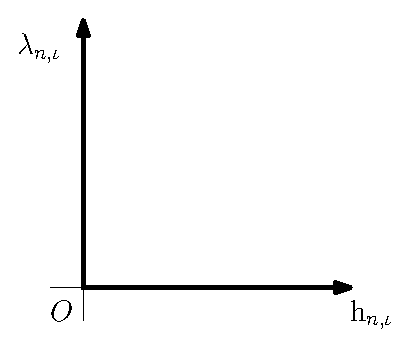
\includegraphics[width=\linewidth]{signorinicontact.eps}
\caption{}\label{fig:appsignorinicontact}
\end{subfigure}
\qquad
\begin{subfigure}{0.3\textwidth}
\centering
\includegraphics[width=\linewidth]{newtonimpact.eps}
\caption{}\label{fig:appnewtonimpact}
\end{subfigure}
\caption{In \textnormal{(a)} Signorini's contact law and in \textnormal{(b)} Newton's impact law without restitution.}
\end{figure}

\subsection{Coulomb's friction law}
Now we define the normal cone formulation of Coulomb's friction law
\begin{align}
-\vbf_{t,\iota} \in N_{C_{t,\iota}}(\lambdab_{t,\iota})\quad \forall \iota\in\Ic_a,\quad \text{with }C_{t,\iota}(\lambda_{n,\iota}) = \{\lambdab_{t,\iota}\ |\ ||\lambdab_{t,\iota}|| \leq \mu\lambda_{n,\iota}\},
\end{align}
which is illustrated in Figure~\ref{fig:appfrictiondisk}.  

\begin{figure}[h]
\centering
\includegraphics[width=.4\textwidth]{frictiondisk.eps}\caption{The friction disk with two seperate friction forces $\lambdab_{t,1}$ and $\lambdab_{t,2}$. $\lambdab_{t,1} = \mu\lambda_{n,1}$, resulting in a tangential velocity $\vbf_{t,\iota}>0$. $\lambdab_{t,2}<\mu\lambda_{n,2}$, leading to a tangential velocity $\vbf_{t,\iota}=0$.}\label{fig:appfrictiondisk}
\end{figure}

$C_t$ is the set of all admitted friction forces. The tangential velocity $\vbf_{t,\iota}$ is directed opposite to the friction force $\lambdab_{t,\iota}$ for isotropic friction. 

Now using the fact that
\begin{align}
\xb = \prox_C(\xb -r\yb), r > 0\ \iff\ -\yb\in N_C(\xb),
\end{align}
we can rewrite the normal cone to a proximal point formulation
\begin{align}
\lambdab_{t,\iota} = \prox_{C_{t,\iota}}(\lambdab_{t,\iota} - r\vbf_{t,\iota})\,\quad\text{with }C_{t,\iota}(\lambda_{n,\iota}) = \{\lambdab_{t,\iota}\ |\ ||\lambdab_{t,\iota}|| \leq \mu\lambda_{n,\iota}\}\text{ and }r>0.
\end{align}
Similarly, for the impact dynamics we can formulate
\begin{align}
\Lambdab_{t,\iota} = \prox_{C_{t,\iota}}(\Lambdab_{t,\iota} - r\vbf^+_{t,\iota})\,\quad \text{with }C_{t,\iota}(\lambda_{n,\iota}) = \{\Lambdab_{t,\iota}\ |\ ||\Lambdab_{t,\iota}|| \leq \mu\Lambda_{n,\iota}\}\text{ and }r>0.
\end{align}

\subsection{System dynamics with contact law and friction law}
The flow dynamics is then described by
\begin{align}
&\Mb(\qb)\dot{\nub} + \Hb(\qb,\nub) = \Sb(\qb)\ub + \sum_{i\in\Ic_c}\left(\wb_{n,\iota}(\qb)\lambda_{n,\iota} + \Wb_{t,\iota}(\qb)\lambdab_{t,\iota} \right), \label{eq:proxcontact1}\\
&\lambda_{n,\iota} = \prox_{C_{n,\iota}}(\lambda_{n,\iota} - rh_{n,\iota}),\label{eq:proxcontact2}\\
&\lambdab_{t,\iota} = \prox_{C_{t,\iota}}(\lambdab_{t,\iota} - r\vbf_{t,\iota}),\label{eq:proxcontact3}
\end{align}
with
\begin{align}
&C_{n,\iota} = (\Rbb^n)^+\text{ and } r>0,\\
&C_{t,\iota}(\lambda_{n,\iota}) = \{\lambdab_{t,\iota}\ |\ ||\lambdab_{t,\iota}|| \leq \mu\lambda_{n,\iota}\}\text{ and }r>0.
\end{align}
The impulsive dynamics that take place when a contact point opens or closes contact is described by
\begin{align}
&\Mb(\qb)(\nub^+ - \nub^-) = \sum_{\iota\in\Ic_c}\left( \wb_{n,\iota}(\qb)\Lambda_{n,\iota} + \Wb_{t,\iota}(\qb)\Lambdab_{t,\iota}\right), \label{eq:proximpact1}\\
&\Lambda_{n,\iota} = \prox_{C_{n,\iota}}(\Lambda_{n,\iota} - r\zeta^+_{n,\iota}),\label{eq:proximpact2}\\
&\Lambdab_{t,\iota} = \prox_{C_{t,\iota}}(\Lambdab_{t,\iota} - r\vbf^+_{t,\iota})\,\label{eq:proximpact3}
\end{align}
with
\begin{align}
&C_{n,\iota} = (\Rbb^n)^+\text{ and } r>0,\\
&C_{t,\iota}(\lambda_{n,\iota}) = \{\Lambdab_{t,\iota}\ |\ ||\Lambdab_{t,\iota}|| \leq \mu\Lambda_{n,\iota}\}\text{ and }r>0.
\end{align}

%% New chapter %%
\pagestyle{fancyreport}
\cleartooddpage
\pagestyle{fancyreport}
\chapter{Frictional Impacts in Mechanical Systems}
\section{Reference trajectories with impact away from slip-stick border}\label{app:impactsaway}
Let us now look at the case where a contact point goes from open to closed away from $\Gamma = 0$, where $\Gamma = 0$ represents the stick/slip border. This is illustrated in Figure~\ref{fig:impactfromborder}. The goal is to prove that for an event away from $\Gamma$, a sufficiently small perturbation cannot cause the trajectory to hit $\gamma = 0$ at a perturbed ante-impact state $\xb^-(t^\epsilon)$ where $\Gamma$ changes sign in comparison with the unperturbed ante-impact state $\alphab^-(\tau)$. From \cite[p. 6]{Rijnen2018} we know that based on the continuity property of $\gamma$ and $\fb$, the perturbed impact state can be written as

\begin{align}
\xb(t^\epsilon) = \alphab(\tau) + \epsilon\dot{\alphab}(\tau)\frac{\partial t^\epsilon}{\partial \epsilon} + \epsilon\zb(\tau) + o(\epsilon),\label{eq:appxpert}
\end{align}
for sufficiently small $\epsilon$. The shortest distance between $\Gamma = \Gamma(\alphab(\tau))$ and $\Gamma = 0$ on the manifold where $\gamma = 0$ is defined as the constant $\delta_{\Gamma}$, which is also illustrated in Figure~\ref{fig:impactfromborder}.

\begin{figure}[h]
\centering
\includegraphics[width=.5\textwidth,trim={0cm 2.5cm 2cm 2.4cm},clip]{impactfromborder.eps}\caption{The guard functions $\gamma$ and $\Gamma$ in the state space of $\qb$. A transition from open to closed is made away from $\Gamma$. $\alphab(t)$ is the nominal trajectory and $\xb(t)$ a perturbed trajectory of the contact point up to the transition.} \label{fig:impactfromborder}
\end{figure}

Let's define a point in the state $\xb_{\gamma=0,\Gamma=0}$ where $\gamma(\xb_{\gamma=0,\Gamma=0})=0$ and $\Gamma(\xb_{\gamma=0,\Gamma=0})=0$. We are evaluating nominal trajectories which impact away from $\Gamma = 0$, i.e. $\Gamma(\alphab(\tau))\neq \Gamma(\xb_{\gamma=0,\Gamma=0})$. Since $\Gamma$ is continuously differentiable, we know
\begin{align}
||\Gamma(\alphab(\tau)) - \Gamma(\xb_{\gamma=0,\Gamma=0})||\leq \kappa||\alphab(\tau)-\xb_{\gamma=0,\Gamma=0}||,\label{eq:appLipschitz2}
\end{align}
where $\kappa>0$ \cite{Leine2008}. Now, since $\Gamma(\alphab(\tau))\neq \Gamma(\xb_{\gamma=0,\Gamma=0})$, we know that $||\Gamma(\alphab(\tau)) - \Gamma(\xb_{\gamma=0,\Gamma=0})||>0$ and therefore from \eqref{eq:appLipschitz2} that $||\alphab(\tau)-\xb_{\gamma=0,\Gamma=0}||>0$, i.e. $\delta_{\Gamma} >0$. Finally, from \eqref{eq:appxpert}, we find

\begin{align}
||\xb(t^\epsilon) - \alphab(\tau)|| = ||\epsilon\dot{\alphab}(\tau)\frac{\partial t^\epsilon}{\partial \epsilon} + \epsilon\zb(\tau) + o(\epsilon)||.
\end{align}
Since $\delta_{\Gamma} > 0$ and $\lim_{\epsilon\rightarrow 0}||\xb(t^\epsilon) - \alphab(\tau)||=0$, there always exists an $\epsilon$ such that $||\xb(t^\epsilon) - \alphab(\tau)||<\delta_{\Gamma}$. 

In other words, this proves that if $\fb$, $\gamma$ and $\Gamma$ are continuous and the nominal trajectory makes impact away from the slip-stick post-impact mode border $\Gamma = 0$, then there always exists a range of $\epsilon$ such that the perturbed state will have the same post-impact mode as the nominal trajectory.

\section{Post-impact accelerations in open-to-stick transitions}\label{app:instantslip}
The mode transition from stick to slip happens when a guard is triggered at acceleration level, 
\begin{align}
\gamma^{\text{st}\rightarrow\text{sl}} = \mu_{\iota}^2\lambda_{n,\iota}^2 - \lambdab_{t,\iota}\lambdab_{t,\iota}^T,
\end{align}
and the post-impact mode is determined by the guard functions defined at velocity level
\begin{align}
\Gamma^{\text{st}\rightarrow\text{sl}}_{\iota} &= \mu_{\iota}^2\Lambda_{n,\iota}^2 - \Lambdab_{t,\iota}\Lambdab_{t,\iota}^T,\\
\Gamma^{\text{sl}\rightarrow\text{st}}_{\iota} &= (\vbf^+_{t,\iota})^T\vbf^+_{t,\iota}.
\end{align}
Since the jump map from open to stick is
\begin{align}
&\Mb(\qb)(\dot{\qb}^+ - \dot{\qb}^-) = \wb_{n,\iota}(\qb)\Lambda_{n,\iota} + \Wb_{t,\iota}(\qb)\Lambdab_{t,\iota},\label{eq:appjump8}\\
&\vrm_{n,\iota}^+ = 0,\label{eq:appjump9}\\
&\vbf_{t,\iota}^+ = 0,\label{eq:appjump10}
\end{align}
which is on velocity level, the post-impact reaction forces of the open-to-stick event can be in the stick-to-slip jump set, causing an immediate transition to slip. This is demonstrated using the flow dynamics of the stick mode at the time-instant of the transition,
\begin{align}
&\Mb(\qb^+)\ddot{\qb}^+ + \Hb(\qb^+,\dot{\qb}^+) = \Sb(\qb^+)\ub^+ + \sum_{\iota\in\Ic_c}\left(\wb_{n,\iota}(\qb^+)\lambda^+_{n,\iota} + \Wb_{t,\iota}(\qb^+)\lambdab^+_{t,\iota} \right), \label{eq:appstickdyn+1}\\
&\wb^T_{n,\iota}(\qb^+)\ddot{\qb}^+ + \dot{\wb}^T_{n,\iota}(\qb^+)\dot{\qb}^+ = 0,\label{eq:appstickdyn+2}\\
&\Wb^T_{t,\iota}(\qb^+)\ddot{\qb}^+ + \dot{\Wb}^T_{t,\iota}(\qb^+)\dot{\qb}^+ = 0.\label{eq:appstickdyn+3}
\end{align}

We can deduce from \eqref{eq:appjump9}-\eqref{eq:appjump10} and \eqref{eq:appstickdyn+2}-\eqref{eq:appstickdyn+3} that the normal acceleration of the transition contact point $\wb^T_{n,\iota}(\qb^+)\ddot{\qb}^+$ and the tangential acceleration of the transitioning contact point $\Wb^T_{t,\iota}(\qb^+)\ddot{\qb}^+$ are both equal to zero. From \eqref{eq:appstickdyn+1} we then notice that $\lambda_{n,\iota}^+$ and $\lambdab_{t,\iota}^+$ depend continuously on $\ub^+$ and can therefore instantly lead to $\mu_{\iota}^2\lambda_{n,\iota}^2 - \lambdab_{t,\iota}\lambdab_{t,\iota}^T>0$ for certain $\ub^+$. For these inputs the contact point will immediately start slipping after the open-to-stick transition. These areas are illustrated in Figure~\ref{fig:stickimmedslip}

\begin{figure}[h]
\centering
\includegraphics[width=.55\textwidth]{stickimmedslip.eps}\caption{The border between an open-to-stick event that stays in stick and an open-to-stick event that immediately starts slipping is illustrated in this figure. The post event state and input indicated in the figure is in the $\mu_{\iota}^2(\lambda^+_{n,\iota})^2 - \lambdab^+_{t,\iota}(\lambdab^+_{t,\iota})^T > 0$ area, causing the contact point to immediately start slipping.} \label{fig:stickimmedslip}
\end{figure}

Using the continuity of the system's flow dynamics and the function $\mu_{\iota}^2(\lambda^+_{n,\iota})^2 - \lambdab^+_{t,\iota}(\lambdab^+_{t,\iota})^T$, we can show that if we choose $\mub^+$ such that $\alphab^+,\mub^+$ is not on $\mu_{\iota}^2(\lambda^+_{n,\iota})^2 - \lambdab^+_{t,\iota}(\lambdab^+_{t,\iota})^T = 0$ then there always exists a range of perturbations $\epsilon$ such that the perturbed post-impact is on the same side of $\mu_{\iota}^2(\lambda^+_{n,\iota})^2 - \lambdab^+_{t,\iota}(\lambdab^+_{t,\iota})^T = 0$ as the unperturbed trajectory similarly to Section~\ref{app:impactsaway}.

%% New chapter %%
\pagestyle{fancyreport}
\cleartooddpage
\pagestyle{fancyreport}
\chapter{Sensitivity Analysis for Input-Dependent Guards}\label{app:Csensitivity}
\section{Linearized jump gain for isolated events}
The perturbed state is defined as
\begin{align}
\xb(t,\epsilon) = \xb(t_0,\epsilon) + \int_{t_0}^{t}\fb(\xb(s,\epsilon),\ub(s,\epsilon),s)ds.
\end{align}
Then
\begin{align}
\frac{\partial\xb(t,\epsilon)}{\partial\epsilon} &= \frac{\partial\xb_0}{\partial\epsilon} + \int_{t_0}^{t}\left(\frac{\partial\fb}{\partial\xb}\frac{\partial\xb}{\partial\epsilon} + \frac{\partial\fb}{\partial\ub}\frac{\partial\ub}{\partial\epsilon}\right)ds,\\
\frac{\partial^2\xb}{\partial t\partial\epsilon} &= \frac{\partial\fb}{\partial\xb}\frac{\partial\xb}{\partial\epsilon} + \frac{\partial\fb}{\partial\ub}\frac{\partial\ub}{\partial\epsilon},
\end{align}
which we can write as
\begin{align}
\frac{\partial^2\xb}{\partial t\partial\epsilon} = D_1\fb(\xb(t,\epsilon),\ub(t,\epsilon),t)\cdot \frac{\partial\xb}{\partial\epsilon} + D_2\fb(\xb(t,\epsilon),\ub(t,\epsilon),t)\cdot \frac{\partial\ub}{\partial\epsilon}, \label{eq:dxdtde}
\end{align}
with $D_i\fb$ the derivative of $\fb$ wrt the $i$th term of $\fb$. Evaluating \eqref{eq:dxdtde} at $\epsilon = 0$ results in the flow dynamics of the positive homogenization
\begin{align}
\dot{\zb} = D_1\fb(\alphab(t),\mub(t),t)\cdot \zb(t) + D_2\fb(\alphab(t),\mub(t),t)\cdot \vb(t),
\end{align}
where 
\begin{align}
\zb(t) = \left.\frac{\partial\xb(t,\epsilon)}{\partial\epsilon}\right|_{\epsilon=0},\text{ and } \vb(t) = \left.\frac{\partial\ub(t,\epsilon)}{\partial\epsilon}\right|_{\epsilon=0} .
\end{align}
When we consider a single jump
\begin{align}
\xb^{+}(t^\epsilon,\epsilon) = \gb(\xb^{-}(t^\epsilon,\epsilon),t^\epsilon),\label{eq:g}
\end{align}
using a Taylor approximation on the left-hand side of \eqref{eq:g} with respect to $\epsilon$ and around $\epsilon = 0$, we can write
\begin{align}
\xb^{+}(t^\epsilon,\epsilon) &= \alphab^{+}(t^\epsilon) + \epsilon \zb^{+}(t^\epsilon) + o(\epsilon),\label{eq:xe}\\
\ub^{+}(t^\epsilon,\epsilon) &= \mub^{+}(t^\epsilon) + \epsilon \vb^{+}(t^\epsilon) + o(\epsilon),\label{eq:ue}
\end{align}
where $\alphab(t)$ is a nominal reference trajectory that satisfies the dynamics of the system and $\mub(t)$ an input that achieves this reference trajectory. Now we expand this in terms of $\epsilon$, so with
\begin{align}
\Delta = \left.\frac{\partial t^\epsilon}{\partial\epsilon}\right|_{\epsilon=0},
\end{align} 
we get
\begin{align}
\alphab^{+}(t^\epsilon) &= \alphab^{+}(\tau) + \epsilon \dot{\alphab}^{+}(\tau)\Delta + o(\epsilon),\\
\mub^{+}(t^\epsilon) &= \mub^{+}(\tau) + \epsilon \dot{\mub}^{+}(\tau)\Delta + o(\epsilon),\\
\zb^{+}(t^\epsilon) &= \zb^{+}(\tau) + \epsilon \dot{\zb}^{+}(\tau)\Delta + o(\epsilon),\\
\vb^{+}(t^\epsilon) &= \vb^{+}(\tau) + \epsilon \dot{\vb}^{+}(\tau)\Delta + o(\epsilon),
\end{align}
which when substituted into \eqref{eq:xe} and \eqref{eq:ue} gives,
\begin{align}
\xb^{+}(t^\epsilon,\epsilon) &= \alphab^{+}(\tau) + \epsilon \dot{\alphab}^{+}(\tau)\Delta + \epsilon \zb^{+}(\tau) + o(\epsilon). \label{eq:xeexp}\\
\ub^{+}(t^\epsilon,\epsilon) &= \mub^{+}(\tau) + \epsilon \dot{\mub}^{+}(\tau)\Delta + \epsilon \vb^{+}(\tau) + o(\epsilon). \label{eq:ueexp}
\end{align}
 To find $\Delta$, we evaluate the ante impact guard function
\begin{align}
\gamma^{-}( \xb^{-}(t^\epsilon),\ub^{-}(t^\epsilon),t^\epsilon) = 0.
\end{align}
In previous work, the guard function $\gamma$ was not dependent on $\ub(t^\epsilon)$ because friction and release was not considered. We now expand $\gamma(\xb(t^\epsilon),\ub(t^\epsilon),t^\epsilon)$ wrt $\epsilon$, giving
\begin{align}
\gamma&(\xb(t^\epsilon),\ub(t^\epsilon),tt^\epsilon) = \gamma( \alphab(\tau), \mub(\tau),\tau) + \epsilon\left[\frac{\partial \gamma}{\partial\epsilon}(\alphab(\tau),\mub(\tau),\tau)\right]_{\epsilon=0} + o(\epsilon),\\
&= \gamma( \alphab(\tau), \mub(\tau),\tau) + \epsilon\left[ \frac{\partial\gamma}{\partial\xb}\left(\frac{\partial\xb}{\partial\epsilon} + \frac{\partial\xb}{\partial tt^\epsilon}\frac{d t^\epsilon}{d\epsilon}\right) + \frac{\partial\gamma}{\partial\ub}\left(\frac{\partial\ub}{\partial\epsilon} + \frac{\partial\ub}{\partial t^\epsilon}\frac{d t^\epsilon}{d\epsilon}\right) + \frac{\partial\gamma}{\partial t^\epsilon}\frac{d t^\epsilon}{d\epsilon}  \right]_{\epsilon=0} + o(\epsilon). \label{eq:gamma}
\end{align}
By definition $\gamma(\tau) = 0$, so we can rewrite \eqref{eq:gamma} to
\begin{align}
\gamma&(\xb(t^\epsilon),\ub(t^\epsilon),t^\epsilon) = \epsilon\left[ D_1 \gamma\cdot \left( \overline{\zb}(\tau) + \dot{\alphab}(\tau)\Delta\right) + D_2 \gamma\cdot  \left( \overline{\vb}(\tau) + \dot{\mub}(\tau) \Delta\right) + D_3\cdot  \gamma \Delta \right]\label{eq:gamma2}
\end{align}

Now we can evaluate \eqref{eq:gamma} using \eqref{eq:gamma2}, which gives
\begin{align}
\epsilon\left[ D_1 \gamma^{-}\cdot \left(\zb^{-}(\tau) + \dot{\alphab}^{-}(\tau)\Delta\right) + D_2 \gamma^{-}\cdot  \left(\vb^{-}(\tau) + \dot{\mub}^{-}(\tau) \Delta\right) + D_3 \gamma^{-}\cdot  \Delta \right] = 0. \label{eq:gamma3}
\end{align}
From \eqref{eq:gamma3} we can determine the expression for $\Delta$,
\begin{align}
\Delta = -\frac{D_1 \gamma^{-} \cdot \zb^{-}(\tau) + D_2 \gamma^{-}\cdot \vb^{-}(\tau)}{\dot{\gamma}^{-}}, \label{eq:Delta}
\end{align}
with
\begin{align}
\gamma^{-} &= \gamma^{-}(\alphab^{-}(\tau),\mub^{-}(\tau),\tau),\\
\dot{\gamma}^{-} &= D_1 \gamma^{-} \cdot \dot{\alphab}^{-} + D_2 \gamma^{-}\cdot  \dot{\mub}^{-} + D_3 \gamma^{-}.
\end{align}

To find the expression for the right hand side of \eqref{eq:g}, we now expand $\gb(\xb^{-}(t^\epsilon,\epsilon),\ub^{-}(t^\epsilon,\epsilon),t^\epsilon)$ with respect to $\epsilon$ as

\begin{align}
\gb(\xb^{-},\ub^{-},t^\epsilon) &= \gb(\alphab^-(\tau),\tau) + \epsilon\left[\frac{\partial\gb}{\partial\epsilon}\right] + o(\epsilon),\\
&= \alphab^+(\tau) + \epsilon\left[\frac{\partial\gb}{\partial\xb}\left(\frac{\partial\xb}{\partial\epsilon} + \frac{\partial\xb}{\partial t^\epsilon}\frac{dt^\epsilon}{d\epsilon} \right) + \frac{\partial\gb}{\partial\ub}\left(\frac{\partial\ub}{\partial\epsilon} + \frac{\partial\ub}{\partial t^\epsilon}\frac{d t^\epsilon}{d\epsilon}\right) + \frac{\partial\gb}{\partial t^\epsilon}\frac{d t^\epsilon}{d\epsilon} \right]_{\epsilon = 0} + o(\epsilon),\\
&= \alphab^+(\tau) + \epsilon\left[D_1\gb\cdot \left(\zb^- + \dot{\alphab}^-\Delta\right) + D_2\gb\cdot \left(\vb^- + \dot{\mub}(\tau) \Delta\right) + D_3\gb\cdot \Delta\right] + o(\epsilon).\label{eq:gexp}
\end{align}

For small $\epsilon$, we can rewrite \eqref{eq:g}, \eqref{eq:Delta} and \eqref{eq:gexp} to a general jump map with counter $k$ as
\begin{align}
\xb^{+}(t^\epsilon,\epsilon) &= \gb(\xb^{-},\ub^{-},t^\epsilon)=:\gb^-,\label{eq:gmulti}\\
\Delta &= -\frac{D_1 \gamma\cdot \zb^-(\tau) + D_2 \gamma\cdot \vb^-(\tau)}{\dot{\gamma}}, \label{eq:Deltamulti}\\
\gb^- &= \alphab^+(\tau) + \epsilon\left[D_1\gb^-\cdot \left(\zb^- (\tau) + \dot{\alphab}^{-}\Delta \right) + D_2\gb^-\cdot \left(\vb^- (\tau) + \dot{\mub}^-\Delta \right) + D_3\gb^-\cdot \Delta \right].\label{eq:gexpmulti}
\end{align}

From \eqref{eq:xeexp} we get
\begin{align}
\zb^+(\tau) = \frac{1}{\epsilon}\left(\xb^{+}(t^\epsilon) - \alphab^+(\tau)\right) -\dot{\alphab}^+(\tau)\Delta,\label{eq:zmulti}
\end{align}
and by equating \eqref{eq:gmulti} and \eqref{eq:gexpmulti} we find an expression for $\overline{\xb}^{+}(t^\epsilon,\epsilon)$ which we can substitute into \eqref{eq:zmulti} resulting in
\begin{align}
\zb^+(\tau) = D_1\gb^-\cdot\left(\zb^- (\tau) + \dot{\alphab}^-\Delta \right) + D_2\gb^-\cdot \left(\vb^- (\tau) + \dot{\mub}^-\Delta \right) + D_3\gb^-\cdot\Delta -\dot{\alphab}^-(\tau)\Delta. \label{eq:zmulti2}
\end{align}

Now, by substituting \eqref{eq:Deltamulti} into \eqref{eq:zmulti2}, we get
\begin{multline}
\zb^+(\tau) = - \left(D_1\gb^-\cdot \fb^{-} + D_2\gb^-\cdot \dot{\mub}^- + D_3\gb^-\cdot 1 - \fb^+\right)\frac{D_1\gamma^-\cdot\zb^- + D_2\gamma^-\cdot\vb^-}{\dot{\gamma}^-}\\ + D_1\gb^-\cdot\zb^- + D_2\gb^-\cdot\vb^-,
\end{multline}
\begin{align}
\zb^+(\tau) = \left(D_1\gb^- - \left(\dot{\gb}^- - \fb^+\right)\frac{D_1\gamma^-}{\dot{\gamma}^-}\right)\cdot\zb^- + \left(D_2\gb^- - \left(\dot{\gb}^- - \fb^+\right)\frac{D_2\gamma^-}{\dot{\gamma}^-}\right)\cdot\vb^-,\label{eq:zmulti3}
\end{align}
with
\begin{align}
\dot{\gb}^- &= D_1\gb^-\cdot \fb^- + D_2\gb^-\cdot \dot{\mub}^- + D_3\gb^-\cdot 1,\\
\fb^+ &=\fb(\alphab^+(\tau),\mub^+(\tau),\tau),\\
\fb^- &=\fb(\alphab^-(\tau),\mub^-(\tau),\tau).
\end{align}
Now, using
\begin{align}
\Gb(\tau) &= D_1\gb^- - \left(\dot{\gb}^- - \fb^+\right)\frac{D_1\gamma^-}{\dot{\gamma}^-},\\
\Jb(\tau) &= D_2\gb^- - \left(\dot{\gb}^- - \fb^+\right)\frac{D_2\gamma^-}{\dot{\gamma}^-},
\end{align}
we can write 
\begin{align}
\zb^+(\tau) &= \Gb\zb^- + \Jb\vb^-.
\end{align}

\section{Linearized jump gain for simultaneous events}\label{app:multjumps}
We now assume that we find the first order approximation of the perturbed post-impact state of two simultaneous jumps, by considering these jumps after each other as
\begin{align}
\ls^{s^{k+1}}\zb(\tau) &= \Gb^{k+1}\ \ls^{s^{k}}\zb + \Jb^{k+1}\ \ls^{s^{k}}\vb\\
\ls^{s^{k+1}}\zb(\tau) &= \Gb^{k+1}\left(\Gb^k\ \ls^{s^{k-1}}\zb + \Jb^k\ \ls^{s^{k-1}}\vb\right) + \Gb^{k+1}\ \ls^{s^{k}}\vb,\\
&= \Gb^{k+1}\Gb^k\ \ls^{s^{k-1}}\zb + \Gb^{k+1}\Jb^k\ \ls^{s^{k-1}}\vb + \Jb^{k+1}\ \ls^{s^{k}}\vb.\label{eq:zkplus}
\end{align}

We prove that this is true by deriving an expression for the post-impact state of two simultaneous jumps, and comparing it with \eqref{eq:zkplus}. Now we evaluate the jump map of two jumps at the same time instant $\tau$,
\begin{align}
\ls^{s^{k+1}}\xb^\epsilon(t^{k+1}) = \ls^{s^{k+1}\leftarrow s^k}\gb(\ls^{s^k}\xb^{\epsilon}(t^{k+1}),\ls^{s^k}\ub^\epsilon(t^{k+1}),t^{k+1}),\label{eq:xe012}
\end{align}
with
\begin{align}
\ls^{s^k}\xb^{\epsilon}(t^{k+1}) = \int_{t^{k}}^{t^{k+1}}\left[\ls^{s^{k}}\fb\left(\ls^{s^{k}}\xb^\epsilon(),\ls^{s^{k}}\ub^\epsilon(t)\right)\right]dt + \ls^{s^{k}}\gb(\ls^{s^{k-1}}\xb^\epsilon(t^{k}),\ls^{s^{k-1}}\ub^\epsilon(t^{k}),t^{k}).\label{eq:xe01}
\end{align}
We rewrite the integral in \eqref{eq:xe01} to
\begin{align}
\int_{t^{k}}^{t^{k+1}}\ \ls^{s^{k}}\fb(t,\epsilon)dt = \Fb(t^{k+1},\epsilon) - \Fb(t^{k},\epsilon) = \Phib(t^{k},t^{k+1},\epsilon),
\end{align}
where $^{s^{k}}\fb\left(\ls^{s^{k}}\xb^\epsilon(t),\ls^{s^{k}}\ub^\epsilon(t)\right)$ can be written as $\ls^{s^{k}}\fb(t,\epsilon)$, because $\xb^\epsilon$ and $\ub^\epsilon$ depend solely on $t$ and $\epsilon$. We now expand $\Phib$ with respect to $\epsilon$, which results in
\begin{align}
\Phib(t^{k},t^{k+1},\epsilon) &= \Phib(\tau^{k},\tau^{k+1},\epsilon) + \epsilon\left.\frac{\partial\Phib}{\partial\epsilon}\right|_{\epsilon = 0} + o(\epsilon),\\
&= \Fb(\tau,0) - \Fb(\tau,0) + \left[\ls^{s^{k}}\fb(t^{k+1},\epsilon)\frac{dt^{k+1}}{d\epsilon} - \ls^{s^{k}}\fb(t^{k+1},\epsilon)\frac{dt^{k}}{d\epsilon} + \int_{t^{k}}^{t^{k+1}}\frac{\partial\ls^{s^{k}}\fb}{\partial\epsilon}dt\right]_{\epsilon=0},\\
&= \ls^{s^{k}}\fb(\Delta^{k+1}-\Delta^{k}), 
\end{align}
since $\tau^k = \tau^{k+1} = \tau$, and $\int_{t^{k}}^{t^{k+1}}\left.\frac{\partial\ls^{s^{k}}\fb(t,\epsilon)}{\partial\epsilon}dt\right|_{\epsilon = 0} = 0$. Here $\ls^{s^{k}}\fb = \ls^{s^{k}}\fb(\ls^{s^{k}}\alphab(\tau),\ls^{s^{k}}\mub(\tau),\tau)$. Note that $\epsilon$ is assumed sufficiently small, such that we can write $t$ as a function of $\epsilon$. By expanding \eqref{eq:xe012} with respect to $\epsilon$, we find
\begin{align}
\ls^{s^{k+1}}\xb^\epsilon(t^{k+1}) = \ls^{s^{k+1}}\alphab(\tau) + \epsilon\left.\frac{\partial\ls^{s^{k+1}}\gb(\ls^{s^{k}}\xb^\epsilon(t^{k+1}),\ls^{s^{k}}\ub^\epsilon(t^{k+1}),t^{k+1})}{\partial\epsilon}\right|_{\epsilon=0} + o(\epsilon),\label{eq:xe012exp}
\end{align}
with
\begin{align}
\left.\frac{\partial\ls^{s^{k+1}}\gb}{\partial\epsilon}\right|_{\epsilon=0} = \left[\frac{\partial\ls^{s^{k+1}}\gb}{\partial\xb}\left(\frac{\partial\ls^{s^k}\xb}{\partial\epsilon} + \frac{\partial\ls^{s^k}\xb}{\partial t}\frac{\text{d} t^{k+1}}{\text{d}\epsilon}\right) + \frac{\partial\ls^{s^{k+1}}\gb}{\partial\ub}\left(\frac{\partial\ls^{s^k}\ub}{\partial\epsilon} + \frac{\partial\ls^{s^k}\ub}{\partial t}\frac{\text{d} t^{k+1}}{\text{d}\epsilon}\right) + \frac{\partial\ls^{s^{k+1}}\gb}{\partial t}\frac{\text{d} t^{k+1}}{\text{d}\epsilon}\right]_{\epsilon=0},
\end{align}
\begin{multline}
\left.\frac{\partial\ls^{s^{k+1}}\gb}{\partial\epsilon}\right|_{\epsilon=0} = \left[D_1\ls^{s^{k+1}}\gb\left(\frac{\partial \Phib}{\partial\epsilon} + D_1\ls^{s^{k}}\gb\left(\frac{\partial\ls^{s^{k-1}}\xb}{\partial\epsilon} + \frac{\partial\ls^{s^{k-1}}\xb}{\partial t}\frac{\text{d}t^{k}}{\text{d}\epsilon}\right) + D_2\ls^{s^{k}}\gb\left(\frac{\partial\ls^{s^{k-1}}\ub}{\partial\epsilon} + \frac{\partial\ls^{s^{k-1}}\ub}{\partial t}\frac{\text{d} t^{k}}{\text{d}\epsilon}\right)\right.\right.\\\left.\left. + D_3\ls^{s^{k}}\gb\frac{\text{d} t^k}{\text{d} \epsilon} \right) + D_2\ls^{s^{k+1}}\gb\left(\frac{\partial\ls^{s^k}\ub}{\partial\epsilon} + \frac{\partial\ls^{s^k}\ub}{\partial t}\frac{\text{d} t^{k+1}}{\text{d}\epsilon}\right) + D_3\ls^{s^{k+1}}\gb\frac{\text{d} t^{k+1}}{\text{d}\epsilon}\right]_{\epsilon=0},
\end{multline}

%\begin{multline}
%\left.\frac{\partial\ls^{s^{k+1}}\gb}{\partial\epsilon}\right|_{\epsilon=0} = \left[D_1\ls^{s^{k+1}}\gb\left(\frac{\partial \Phib}{\partial\epsilon} + D_1\ls^{s^{k}}\gb\left(\frac{\partial\ls^{s^{k-1}}\xb}{\partial\epsilon} + \frac{\partial\ls^{s^{k-1}}\xb}{\partial t}\frac{\text{d}t^{k}}{\text{d}\epsilon}\right) + D_2\ls^{s^{k}}\gb\left(\frac{\partial\ls^{s^{k-1}}\ub}{\partial\epsilon} + \frac{\partial\ls^{s^{k-1}}\ub}{\partial t}\frac{\text{d} t^{k}}{\text{d}\epsilon}\right)\right.\right.\\\left.\left. + D_3\ls^{s^{k}}\gb\frac{\text{d} t^k}{\text{d} \epsilon} + \frac{\partial\ls^{s^{k}}\xb}{\partial t}\frac{\text{d}t^{k+1}}{\text{d}\epsilon}\right) + D_2\ls^{s^{k+1}}\gb\left(\frac{\partial\ls^{s^k}\ub}{\partial\epsilon} + \frac{\partial\ls^{s^k}\ub}{\partial t}\frac{\text{d} t^{k+1}}{\text{d}\epsilon}\right) + D_3\ls^{s^{k+1}}\gb\frac{\text{d} t^{k+1}}{\text{d}\epsilon}\right]_{\epsilon=0},
%\end{multline}

\begin{multline}
\left.\frac{\partial\ls^{s^{k+1}}\gb}{\partial\epsilon}\right|_{\epsilon=0} = D_1\ls^{s^{k+1}}\gb\cdot\left(\ls^{s^k}\dot{\alphab}(\Delta^{k+1}-\Delta^{k}) + D_1\ls^{s^k}\gb\cdot\left(\ls^{s^{k-1}}\zb+\ls^{s^{k-1}}\dot{\alphab}\Delta^{k}\right) + D_2\ls^{s^k}\gb\cdot\left(\ls^{s^{k-1}}\vb+\ls^{s^{k-1}}\dot{\mub}\Delta^{k}\right) \right. \\ \left. + D_3\ls^{s^k}\gb\cdot\Delta^{k}\right)+ D_2 \ls^{s^{k+1}}\gb\cdot\left(\ls^{s^{k}}\vb+\ls^{s^{k}}\dot{\mub}\Delta^{k+1} \right) + D_3\ls^{s^{k+1}}\gb\cdot\Delta^{k+1}. \label{eq:dg1de}
\end{multline}

%\begin{multline}
%\left.\frac{\partial\ls^{s^{k+1}}\gb}{\partial\epsilon}\right|_{\epsilon=0} = D_1\ls^{s^{k+1}}\gb\cdot\left(\ls^{s^k}\dot{\alphab}(\Delta^{k+1}-\Delta^{k}) + D_1\ls^{s^k}\gb\cdot\left(\ls^{s^{k-1}}\zb+\ls^{s^{k-1}}\dot{\alphab}\Delta^{k}\right) + D_2\ls^{s^k}\gb\cdot\left(\ls^{s^{k-1}}\vb+\ls^{s^{k-1}}\dot{\mub}\Delta^{k}\right) \right. \\ \left. + D_3\ls^{s^k}\gb\cdot\Delta^{k} + \ls^{s^k}\dot{\alphab}\Delta^{k+1}\right)+ D_2 \ls^{s^{k+1}}\gb\cdot\left(\ls^{s^{k}}\vb+\ls^{s^{k}}\dot{\mub}\Delta^{k+1} \right) + D_3\ls^{s^{k+1}}\gb\cdot\Delta^{k+1}. \label{eq:dg1de}
%\end{multline}

We now substitute \eqref{eq:dg1de} into \eqref{eq:xe012exp}, which we in turn substitute into \eqref{eq:zmulti} to get

\begin{multline}
\ls^{s^{k+1}}\zb(\tau) = D_1\ls^{s^{k+1}}\gb\cdot\ls^{s^{k}}\fb\Delta^{k+1} - D_1\ls^{s^{k+1}}\gb\cdot\ls^{s^{k}}\fb\Delta^{k} + D_1\ls^{s^{k+1}}\gb\cdot\left(D_1\ls^{s^{k}}\gb\cdot\left(\ls^{s^{k-1}}\zb+\ls^{s^{k-1}}\fb\Delta^{k}\right)\right.\\
\left.+D_2\ls^{s^{k}}\gb\cdot\left(\ls^{s^{k-1}}\vb+\ls^{s^{k-1}}\dot{\mub}\Delta^{k}\right)+D_3\ls^{s^{k}}\gb\cdot\Delta^{k}\right) + D_2 \ls^{s^{k+1}}\gb\cdot\left(\ls^{s^{k}}\vb+\ls^{s^{k}}\dot{\mub}\Delta^{k+1} \right) + \left(D_3\ls^{s^{k+1}}\gb - \ls^{s^{k+1}}\fb\right)\Delta^{k+1},\label{eq:z2}
\end{multline}
with $\ls^{s^k}\fb = \ls^{s^k}\fb(\ls^{s^k}\alphab(\tau),\ls^{s^k}\mub(\tau),\tau)$. The five terms in \eqref{eq:z2} can be rewritten into
\begin{align}
D_1\ls^{s^{k+1}}\gb\cdot\ls^{s^{k}}\fb\Delta^{k+1} &= -\frac{D_1\ls^{s^{k+1}}\gb\cdot\ls^{s^{k+1}}\fb}{\dot{\gamma}^{k+1}}\left(D_1\gamma^{k+1}\cdot\left(\Gb^{k}\ \ls^{s^{k-1}}\zb+\Jb^{k}\ \ls^{s^{k-1}}\vb\right) +D_2\gamma^{k+1}\cdot\ls^{s^{k}}\vb\right),\\
-D_1\ls^{s^{k+1}}\gb\cdot\ls^{s^{k}}\fb\Delta^{k} &= \frac{D_1\ls^{s^{k+1}}\gb\cdot\ls^{s^{k}}\fb}{\dot{\gamma}^{k}}\left(D_1\gamma^{k}\cdot\ls^{s^{k-1}}\zb + D_2\gamma^{k}\cdot\ls^{s^{k-1}}\vb\right),
\end{align}
\begin{multline}
D_1\ls^{s^{k+1}}\gb\cdot\left(D_1\ls^{s^{k}}\gb\cdot\left(\ls^{s^{k-1}}\zb + \ls^{s^{k-1}}\fb\Delta^{k}\right) + D_2\ls^{s^{k}}\gb\cdot\left(\ls^{s^{k-1}}\vb+\ls^{s^{k-1}}\dot{\mub}\Delta^{k}\right) + D_3\ls^{s^{k}}\gb\cdot\Delta^{k}\right) = \\
D_1\ls^{s^{k+1}}\gb\cdot\left(-\frac{D_1\ls^{s^{k}}\gb\cdot\ls^{s^{k-1}}\fb}{\dot{\gamma}^{k}}D_1\gamma^{k} - \frac{D_2\ls^{s^{k}}\gb\cdot\ls^{s^{k-1}}\dot{\mub}}{\dot{\gamma}^{k}}D_1\gamma^{k} - \frac{D_3\ls^{s^{k}}\gb\cdot 1}{\dot{\gamma}^{k}}D_1\gamma^{k} + D_1\ls^{s^{k}}\gb\right)\cdot\ls^{s^{k-1}}\zb \\
+ D_1\ls^{s^{k+1}}\gb\cdot\left(-\frac{D_1\ls^{s^{k}}\gb\cdot\ls^{s^{k-1}}\fb}{\dot{\gamma}^{k}}D_2\gamma^{k} - \frac{D_2\ls^{s^{k}}\gb\cdot\ls^{s^{k-1}}\dot{\mub}}{\dot{\gamma}^{k}}D_2\gamma^{k} - \frac{D_3\ls^{s^{k}}\gb\cdot 1}{\dot{\gamma}^{k}}D_2\gamma^{k} + D_2\ls^{s^{k}}\gb \right)\cdot \ls^{s^{k-1}}\vb,
\end{multline}
\begin{multline}
D_2 \ls^{s^{k+1}}\gb\cdot\left(\ls^{s^{k}}\vb+\ls^{s^{k}}\dot{\mub}\Delta^{k+1} \right) = -\frac{D_2\ls^{s^{k+1}}\gb\cdot\ls^{s^k}\dot{\mub}}{\dot{\gamma}^{k+1}}D_1\gamma^{k+1}\cdot\Gb^k\ \ls^{s^{k-1}}\zb -\frac{D_2\ls^{s^{k+1}}\gb\cdot\ls^{s^k}\dot{\mub}}{\dot{\gamma}^{k+1}}D_1\gamma^{k+1}\cdot\Jb^k\ \ls^{s^{k-1}}\vb\\ + \left(D_2\ls^{s^{k+1}}\gb - \frac{D_2\ls^{s^{k+1}}\gb\cdot\ls^{s^k}\dot{\mub}}{\dot{\gamma}^{k+1}}D_2\gamma^{k+1}\right)\cdot\ls^{s^k}\vb,
\end{multline}
\begin{align}
&\left(D_3\ls^{s^{k+1}}\gb\cdot 1 - \ls^{s^{k+1}}\fb\right)\Delta^{k+1} = -\frac{D_3\ls^{s^{k+1}}\gb\cdot 1+\ls^{s^{k+1}}\fb}{\dot{\gamma}^{k+1}}\left(D_1\gamma^{k+1}\cdot\left(\Gb^{k}\ \ls^{s^{k-1}}\zb + \Jb^{k}\ \ls^{s^{k-1}}\vb\right) + D_2\gamma^{k+1}\cdot\ls^{s^{k}}\vb\right).
\end{align}
When we substitute the equations above into \eqref{eq:z2}, after reordering the expression we get
\begin{multline}
\ls^{s^{k+1}}\zb(\tau) = \left(\frac{\ls^{s^{k+1}}\fb - D_1\ls^{s^{k+1}}\gb\cdot\ls^{s^{k}}\fb - D_2\ls^{s^{k+1}}\gb\cdot\ls^{s^{k}}\dot{\mub} - D_3\ls^{s^{k+1}}\gb\cdot 1}{\dot{\gamma}^{k+1}}D_1\gamma^{k+1}\cdot\Gb^{k}\right.\\
\left. + D_1\ls^{s^{k+1}}\gb\cdot\frac{\ls^{s^{k}}\fb - D_1\ls^{s^{k}}\gb\cdot\ls^{s^{k-1}}\fb - D_2\ls^{s^{k}}\gb\cdot\ls^{s^{k-1}}\dot{\mub} - D_3\ls^{s^{k}}\gb\cdot 1}{\dot{\gamma}^{k}}D_1\gamma^{k+1} + D_1\ls^{s^{k+1}}\gb D_1\ls^{s^{k}}\gb\cdot 1\right)\ls^{s^{k-1}}\zb\\
+ \left(\frac{\ls^{s^{k+1}}\fb-D_1\ls^{s^{k+1}}\gb\cdot\ls^{s^{k}}\fb -D_2\ls^{s^{k+1}}\gb\cdot\ls^{s^{k}}\dot{\mub} - D_3\ls^{s^{k+1}}\gb\cdot 1}{\dot{\gamma}^{k+1}}D_1\gamma^{k+1}\cdot\Jb^{k}\right.\\
\left. + D_1\ls^{s^{k+1}}\gb\cdot\frac{\ls^{s^{k}}\fb-D_1\ls^{s^{k}}\gb\cdot\ls^{s^{k-1}}\fb-D_2\ls^{s^{k}}\gb\cdot\ls^{s^{k-1}}\dot{\mub}-D_3\ls^{s^{k}}\gb\cdot 1}{\dot{\gamma}^{k}}D_2\gamma^{k+1} + D_1\ls^{s^{k+1}}\gb D_2\ls^{s^{k}}\gb\cdot 1 \right)\ls^{s^{k-1}}\vb\\
+ \left(\frac{\ls^{s^{k+1}}\fb-D_1\ls^{s^{k+1}}\gb\cdot\ls^{s^{k}}\fb - D_2\ls^{s^{k+1}}\gb\cdot\ls^{s^{k}}\dot{\mub} - D_3\ls^{s^{k+1}}\gb\cdot 1}{\dot{\gamma}^{k+1}}D_2\gamma^{k+1}\right)\ls^{s^{k}}\vb,
\end{multline}
from which we can isolate $\Gb^{k}$, and $\Jb^{k}$ resulting in
\begin{multline}
\ls^{s^{k+1}}\zb(\tau) = \left(\frac{\ls^{s^{k+1}}\fb - D_1\ls^{s^{k+1}}\gb\cdot\ls^{s^{k}}\fb  - D_2\ls^{s^{k+1}}\gb\cdot\ls^{s^{k}}\dot{\mub} - D_3\ls^{s^{k+1}}\gb\cdot 1}{\dot{\gamma}^{k+1}}D_1\gamma^{k+1} + D_1\ls^{s^{k+1}}\gb\cdot 1\right)\Gb^{k}\ \ls^{s^{k-1}}\zb\\
+ \left(\frac{\ls^{s^{k+1}}\fb - D_1\ls^{s^{k+1}}\gb\cdot\ls^{s^{k}}\fb - D_2\ls^{s^{k+1}}\gb\cdot\ls^{s^{k}}\dot{\mub} - D_3\ls^{s^{k+1}}\gb\cdot 1}{\dot{\gamma}^{k+1}}D_1\gamma^{k+1} + D_1\ls^{s^{k+1}}\gb\cdot 1\right)\Jb^{k}\ \ls^{s^{k-1}}\vb \\
+ \left(\frac{\ls^{s^{k+1}}\fb-D_1\ls^{s^{k+1}}\gb\cdot\ls^{s^{k}}\fb - D_2\ls^{s^{k+1}}\gb\cdot\ls^{s^{k}}\dot{\mub} - D_3\ls^{s^{k+1}}\gb\cdot 1}{\dot{\gamma}^{k+1}}D_2\gamma^{k+1} + D_2\ls^{s^{k+1}}\gb\cdot 1\right)\ls^{s^{k}}\vb,
\end{multline}
which is equal to
\begin{align}
&\ls^{s^{k+1}}\zb(\tau) = \Gb^{k+1}\Gb^k\ \ls^{s^{k-1}}\zb + \Gb^{k+1}\Jb^k\ \ls^{s^{k-1}}\vb + \Jb^{k+1}\ \ls^{s^{k}}\vb.\label{eq:zkplusfinal}
\end{align}

Here we see that \eqref{eq:zkplusfinal} is equal to \eqref{eq:zkplus}. This proves that for any $k$, the first-order approximation of the post-impact state of two simultaneous jumps at $\tau$ can be found by evaluating the two jumps separately. Since $k$ is a variable in this proof, using an induction-like proof, this holds for any amount of jumps as well. This is illustrated in Figure~\ref{fig:kjumps}. 

\begin{figure}[bt!]
\centering
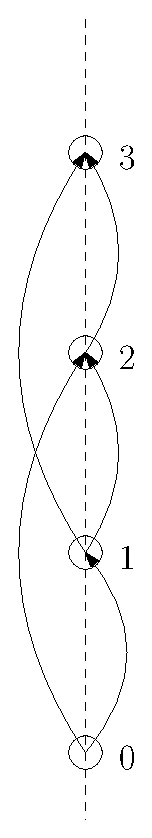
\includegraphics[width=.08\textwidth]{kjumps.eps}\caption{This figure illustrates how the derivation of the jump gain for two simultaneous jumps can be extended intuitively to a jump gain for an arbitrary number of simultaneous jumps.}\label{fig:kjumps}
\end{figure}

When we take $k = 1$, we show that the jumps from $0$ to $2$ can be described by evaluating the jump from $0$ to $1$ and the jump $1$ to $2$ in succession. This also holds for $k = 2$. The jump from $0$ to $3$ can be described by evaluating the jump from $0$ to $2$ and the jump from $2$ to $3$ in succession. This indicates that we can use \eqref{eq:zkplusfinal} to find an expression for the approximation of the post-impact state for $l$ simultaneous jumps, with $l\in \mathbb{Z}$. Also, we show that multiple constant jump gains will result in a total jump which can also be described by a constant jump gain.

Intuitively, for $l$ simultaneous jumps, we can find the approximation of the post-impact state using

\begin{align}
\ls^{l\leftarrow 0}\zb(\tau) = \ls^{l \leftarrow 0}\Lb(\zb^{0}(\tau),\vb(\tau),\tau) = \ls^{l\leftarrow 0}\Gb\zb^{0}(\tau) + \sum_{i=0}^{l-1}\left(\ ^{l\leftarrow i+1}\Gb\ \ls^{i+1 \leftarrow i}\boldsymbol{J}\vb^{i}(\tau)\right),\label{eq:ljumps}
\end{align}

where the superscript
\begin{align}
b\leftarrow a =b\leftarrow (b-1) \leftarrow \cdots \leftarrow (a+1) \leftarrow a,
\end{align}
and
\begin{align}
^{b\leftarrow a}\Gb &=\ ^{b\leftarrow (b-1)}\Gb\cdots\ ^{(a+2)\leftarrow (a+1)}\Gb^{(a+1)\leftarrow a}\Gb,\\
^{b\leftarrow a}\Jb &=\ ^{b\leftarrow (b-1)}\Jb\cdots\ ^{(a+2)\leftarrow (a+1)}\Jb^{(a+1)\leftarrow a}\Jb,
\end{align}
with slight abuse of notation, in the sense that $b-1$ indicates the mode-descriptor that describes the mode before the mode that is desribed by $b$.

\section{Positive homogeneity}\label{app:poshom}
The approximation of the perturbed trajectory $\xb$ can be found using $\alphab + \epsilon\zb$, with

\begin{align}
\ls^{s^{k-1}}\dot{\zb} &=\ls^{s^{k-1}}\Ab(t)\ls^{s^{k-1}}\zb +\ls^{s^{k-1}}\Bb(t)\ls^{s^{k-1}}\vb,\nonumber\\
\ls^{s^{k}}\zb &= \ls^{s^{k}\leftarrow s^{k-1}}\Hb\left(\ls^{s^{k-1}}\zb,\ls^{s^{k-1}}\vb,t\right),\label{eq:PHdyn}\\
\ls^{s^{k}}\dot{\zb} &=\ls^{s^{k}}\Ab(t)\ls^{s^{k}}\zb +\ls^{s^{k}}\Bb(t)\ls^{s^{k-1}}\vb,\nonumber
\end{align}
where
\begin{align}
^{s^{k}}\Ab(t) &= D_1\ls^{s^{k}}\fb\left(\ls^{s^{k}}\alphab(t),\ls^{s^{k}}\mub(t),t\right),\\
^{s^{k}}\Bb(t) &= D_2\ls^{s^{k}}\fb\left(\ls^{s^{k}}\alphab(t),\ls^{s^{k}}\mub(t),t\right).
\end{align}

When we look at \eqref{eq:PHdyn}, the continuous dynamics of the system are linear. Because of the positively homogeneous jump gain $\Hb$ however, this linearity property is lost. We can see this by looking at the general solution of \eqref{eq:PHdyn}. A system $\fb(\xb,\ub,t)$ with state $\xb$ and input $\ub$ is linear if $\fb(\xb_1,\vb_1) + \fb(\xb_2,\vb_2) = \fb(\xb_1+\xb_2,\vb_1+\vb_2)$. The solutions of \eqref{eq:PHdyn} before the jump are in the form of

\begin{align}
\ls^{s^{k-1}}\zb_1(\tau) &= \ls^{s^{k-1}}\phib(t,t_0)\ls^{s^{k-1}}\zb_1(t_0) + \int_{t_0}^\tau \left[\ls^{s^{k-1}}\phib(t,s)\ls^{s^{k-1}}\Bb(s)\vb_1(s)\right]ds,\\
\ls^{s^{k-1}}\zb_2(\tau) &= \ls^{s^{k-1}}\phib(t,t_0)\ls^{s^{k-1}}\zb_2(t_0) + \int_{t_0}^\tau \left[\ls^{s^{k-1}}\phib(t,s)\ls^{s^{k-1}}\Bb(s)\vb_2(s)\right]ds,
\end{align}
with $t_0$ the initial time and $\tau$ the jump time.
When we add these solutions together we find
\begin{multline}
^{s^{k-1}}\zb_1(\tau) + \ls^{s^{k-1}}\zb_2(\tau) = \ls^{s^{k-1}}\phib(t,t_0)\left(\ls^{s^{k-1}}\zb_1(t_0) + \ls^{s^{k-1}}\zb_2(t_0)\right) \\+ \int_{t_0}^\tau \left[\ls^{s^{k-1}}\phib(t,s)\ls^{s^{k-1}}\Bb(s)\left(\vb_1(s) + \vb_2(s)\right)\right]ds,
\end{multline}
which is equal to the solution of $^{s^{k-1}}\zb_3(t_0) = ^{s^{k-1}}\zb_1(t_0) + ^{s^{k-1}}\zb_2(t_0)$ with $\vb_3(t) = \vb_1(t) + \vb_2(t)$, i.e., the linearity property holds. When $^{s^{k-1}}\zb_1$ jumps with $\Gb^1(\zb,\tau)$ and $^{s^{k-1}}\zb_1(\tau)$ jumps with $\Gb^2(\zb,\tau)$ we find the solutions post jump to be
\begin{align}
^{s^{k}}\zb_1(\tau) &= \ls^{s^{k}}\phib(t,t_0)\ \Gb^1(^{s^{k-1}}\zb_1(t_0),\tau) + \int_{t_0}^\tau \left[\ls^{s^{k}}\phib(t,s)\ls^{s^{k}}\Bb(s)\vb_1(s)\right]ds,\label{eq:z1sol}\\
^{s^{k}}\zb_2(\tau) &= \ls^{s^{k}}\phib(t,t_0)\ \Gb^2(^{s^{k-1}}\zb_2(t_0),\tau) + \int_{t_0}^\tau \left[\ls^{s^{k}}\phib(t,s)\ls^{s^{k}}\Bb(s)\vb_2(s)\right]ds,
\end{align}
which when added together results in
\begin{multline}
^{s^{k}}\zb_1(\tau) + \ls^{s^{k}}\zb_2(\tau) = \ls^{s^{k}}\phib(t,t_0)\left(\Gb^1 \ls^{s^{k-1}}\zb_1 + \Jb^1\ls^{s^{k-1}}\vb_1 + \Gb^2 \ls^{s^{k-1}}\zb_2 + \Jb^2\ls^{s^{k-1}}\vb_2\right) \\+ \int_{t_0}^\tau \left[\ls^{s^{k}}\phib(t,s)\ls^{s^{k}}\Bb(s)\left(\vb_1(s) + \vb_2(s)\right)\right]ds.\label{eq:soladd}
\end{multline}
Here we see that the solution of $\ls^{s^{k-1}}\zb_3(t_0) = \ls^{s^{k-1}}\zb_1(t_0) + \ls^{s^{k-1}}\zb_2(t_0)$ with $\vb_3(t) = \vb_1(t) + \vb_2(t)$, which jumps with $\Gb_3(\zb,\tau)$, is only the equal to \eqref{eq:soladd} if $\Gb_1(\zb,\tau) = \Gb_2(\zb,\tau) = \Gb_3(\zb,\tau)$. In other words, the system only maintains its linearity after jump if the jump maps are equal for each ante jump state. Because this is generally not true, we show that the system is positive homogeneous for any jump gains. A system $\fb(\xb,\ub)$ with state $\xb$ and input $\ub$ is called positively homogeneous of order $\kappa$, when $\alpha^{\kappa} \fb(\xb,\ub) = \fb(\alpha \xb, \alpha \ub)$. If we multiply \eqref{eq:z1sol} with a constant $\alpha$, we find
\begin{align}
\ls^{s^{k}}\zb_1(\tau) &= \alpha \ls^{s^{k}}\phib(t,t_0)\ \left(\Gb^1 \ls^{s^{k-1}}\zb_1 + \Jb^1\ls^{s^{k-1}}\vb_1\right) + \alpha\int_{t_0}^\tau \left[\ls^{s^{k}}\phib(t,s)\ls^{s^{k-1}}\Bb(s)\vb_1(s)\right]ds.\label{eq:alphaz1sol}
\end{align}
If we now look at the solution for $\zb_4(t_0) = \alpha\zb_1(t_0)$ with $\vb_4(t) = \alpha\vb_1(t)$ jumping with $\Gb^4(\tau)$, and using the fact that $\Gb^4(\tau) = \Gb^1(\tau)$, we find the same solution as \eqref{eq:alphaz1sol}. This shows that the system \eqref{eq:PHdyn} is positively homogeneous of order zero, for any jump gain $^{s^{k}\leftarrow s^{k-1}}\Hb\left(\ls^{s^{k-1}}\zb,\ls^{s^{k-1}}\zb,t\right)$. Hence the name, positively homogeneous jump gain. 


%% New chapter %%
\pagestyle{fancyreport}
\cleartooddpage
\pagestyle{fancyreport}
\chapter{Trajectory Tracking Visualization}\label{app:simulations}
This chapter visualizes the simulations performed in Section~\ref{sec:5track}. First the reference trajectory is visualized with snapshots of the system performing the nominal motion Figure~\ref{fig:appref}. Then the same visualization is shown in Figure~\ref{fig:apptrack} for a trajectory with an initial state-and-input perturbation, which tracks the reference trajectory.
\begin{figure}[bt!]
%\begin{minipage}[c]{.3\textwidth}
%\centering
%    \includegraphics[width=\textwidth]{reference/frame28.eps}
%	\begin{flushleft}
%    \includegraphics[scale=0.55]{reference/refsnap_t80.eps}
%	\end{flushleft}
%    \includegraphics[width=\textwidth]{tracking/frame28.eps}
%	\begin{flushleft}
%    \includegraphics[scale=0.55]{tracking/trcsnap_t80.eps}
%	\end{flushleft}
%	\caption*{$t=0.800$}
%\end{minipage}
\begin{minipage}[c]{.3\textwidth}
\centering
    \includegraphics[width=\textwidth]{reference/frame29.eps}
	\begin{flushleft}
    \includegraphics[scale=0.55]{reference/refsnap_t87.eps}
	\end{flushleft}
    \includegraphics[width=\textwidth]{tracking/frame29.eps}
	\begin{flushleft}
    \includegraphics[scale=0.55]{tracking/trcsnap_t87.eps}
	\end{flushleft}
	\caption*{$t=0.866$}
\end{minipage}
\begin{minipage}[c]{.3\textwidth}
\centering
    \includegraphics[width=\textwidth]{reference/frame30.eps}
	\begin{flushleft}
    \includegraphics[scale=0.55]{reference/refsnap_t93.eps}
	\end{flushleft}
    \includegraphics[width=\textwidth]{tracking/frame30.eps}
	\begin{flushleft}
    \includegraphics[scale=0.55]{tracking/trcsnap_t93.eps}
	\end{flushleft}
	\caption*{$t=0.933$}
\end{minipage}
\begin{minipage}[c]{.3\textwidth}
\centering
    \includegraphics[width=\textwidth]{reference/frame31.eps}
	\begin{flushleft}
    \includegraphics[scale=0.55]{reference/refsnap_t100.eps}
	\end{flushleft}
    \includegraphics[width=\textwidth]{tracking/frame31.eps}
	\begin{flushleft}
    \includegraphics[scale=0.55]{tracking/trcsnap_t100.eps}
	\end{flushleft}
	\caption*{$t=1.000$}
\end{minipage}

\begin{minipage}[c]{.3\textwidth}
\centering
    \includegraphics[width=\textwidth]{reference/frame32.eps}
	\begin{flushleft}
    \includegraphics[scale=0.55]{reference/refsnap_t103.eps}
	\end{flushleft}
    \includegraphics[width=\textwidth]{tracking/frame32.eps}
	\begin{flushleft}
    \includegraphics[scale=0.55]{tracking/trcsnap_t105.eps}
	\end{flushleft}
	\caption*{$t=1.066$}
\end{minipage}
\begin{minipage}[c]{.3\textwidth}
\centering
    \includegraphics[width=\textwidth]{reference/frame33.eps}
	\begin{flushleft}
    \includegraphics[scale=0.55]{reference/refsnap_t113.eps}
	\end{flushleft}
    \includegraphics[width=\textwidth]{tracking/frame33.eps}
	\begin{flushleft}
    \includegraphics[scale=0.55]{tracking/trcsnap_t113.eps}
	\end{flushleft}
	\caption*{$t=1.133$}
\end{minipage}
\begin{minipage}[c]{.3\textwidth}
\centering
    \includegraphics[width=\textwidth]{reference/frame34.eps}
	\begin{flushleft}
    \includegraphics[scale=0.55]{reference/refsnap_t120.eps}
	\end{flushleft}
    \includegraphics[width=\textwidth]{tracking/frame34.eps}
	\begin{flushleft}
    \includegraphics[scale=0.55]{tracking/trcsnap_t120.eps}
	\end{flushleft}
	\caption*{$t=1.200$}
\end{minipage}
%\begin{minipage}[c]{.3\textwidth}
%\centering
%    \includegraphics[width=\textwidth]{reference/frame35.eps}
%	\begin{flushleft}
%    \includegraphics[scale=0.55]{reference/refsnap_t127.eps}
%	\end{flushleft}
%    \includegraphics[width=\textwidth]{tracking/frame35.eps}
%	\begin{flushleft}
%    \includegraphics[scale=0.55]{tracking/trcsnap_t127.eps}
%	\end{flushleft}
%	\caption*{$t=1.266$}
%\end{minipage}
%\begin{minipage}[c]{.3\textwidth}
%\centering
%    \includegraphics[width=\textwidth]{reference/frame36.eps}
%	\begin{flushleft}
%    \includegraphics[scale=0.55]{reference/refsnap_t133.eps}
%	\end{flushleft}
%    \includegraphics[width=\textwidth]{tracking/frame36.eps}
%	\begin{flushleft}
%    \includegraphics[scale=0.55]{tracking/trcsnap_t133.eps}
%	\end{flushleft}
%	\caption*{$t=1.333$}
%\end{minipage}
\caption{Snapshots of the system in Section~\ref{sec:5sys} performing the reference trajectory in Section~\ref{sec:5track}.}\label{fig:appref}
\end{figure}

% New chapter %%
\pagestyle{fancyreport}
%\cleartooddpage
%\pagestyle{fancyreport}
\chapter{Code of Scientific Conduct}\label{app:conduct}
\begin{center}
\includegraphics[trim={0 0 5cm 0},clip,angle=90,width=.9\textwidth]{codeofconduct.pdf}
\end{center}

%% New chapter %%
%\pagestyle{fancyreport}
%\cleartooddpage
%\pagestyle{fancyreport}
%\chapter{Verification of Assumptions}\label{app:assumptions}

%% New chapter %%
%\pagestyle{fancyreport}
%\cleartooddpage
%\pagestyle{fancyreport}
%\chapter{Simulation Design}\label{app:sim}
%This chapter discusses the numerical validation presented in Chapter~\ref{ch:vali}. First the kinematics and dynamics of the considered system will be presented in Section~\ref{app:kindyn}, which is a RRR-robot opening a door in a planar setting \cite{Rijnen2018b}. Then, the design of the reference trajectory is discussed in Section~\ref{app:trajdesign}. Finally, the sensitivity analysis of the considered system is presented in Section~\ref{app:sens}. Note that the work presented in this chapter and Chapter~\ref{ch:vali} are work in progress, and are merely first steps towards achieving a numerical validation of the theory presented in this work.
%
%\section{Kinematics and dynamics}\label{app:kindyn}
%In this section, the considered system for the numerical validation is presented. The considered system is a robot arm with three revolute joints opening a door, in a planar setting. The equations of motion for that system will be presented in a concise manner. For a more thorough derivation of the equations of motion, the reader is referred to \cite{Rijnen2018b}.
%
%\section{Reference trajectory design}\label{app:trajdesign}
%
%\section{Sensitivity analysis}\label{app:sens}
\end{document}